\chapter{The Image Of Yourself}

This chapter follows J. Krishnamurti's Brockwood Park inquiry into the image of oneself, preserved from the Krishnamurti Foundation Trust source material and curated for this course by LazyingArt LLC through Video2Book. No validated blackboard equations, diagrams, or mathematical screenshots were kept for this lecture. The displayed formulas and TikZ figures below are therefore transcript-backed conceptual notation, not recovered board work. They are used sparingly to hold the inquiry in view: the word and the thing, the divided and undivided movement of consciousness, hurt and image, relationship and no relationship, and the final distinction between method and remaining with the fact.

\section{The Unconscious As A Question}

The lecture opens by returning to the previous concern: human beings need to change, yet do not change. They accept, or continue within, intolerable conditions of the psyche. Krishnamurti does not begin by adding one more explanation to the pile. He turns the inquiry through a different angle: who has invented the unconscious?

That question is deliberately unsettling. The word ``unconscious'' is not first accepted and then analyzed. It is itself placed under observation. Perhaps the word already carries a picture: a hidden chamber, a deeper layer, a storehouse of motives, racial memories, family memories, symbols, dreams, and hints. But if the word has already divided the field, then the first act of inquiry is to notice that division.

The first notation is therefore a warning against notation itself:

\begin{equation}
\text{word} \neq \text{thing}.
\end{equation}

One speaker gives the familiar account fairly. There are actions whose origin we do not see. There are habitual uses of words. There are dreams in which jealousy or some other movement becomes visible. There are slips of the tongue that seem to disclose intention. There are past wounds that govern conduct though one may not know it. The lecture does not need to deny these phenomena. It asks whether the name we give them has misled us.

The conventional picture may be written as a layered model:

\begin{equation}
\mathcal{C}_{\text{surface}} + \mathcal{C}_{\text{hidden}},
\qquad
\mathcal{C}_{\text{hidden}} = \text{``the unconscious''}.
\end{equation}

In that notation, \(\mathcal{C}_{\text{surface}}\) is what one ordinarily calls conscious, and \(\mathcal{C}_{\text{hidden}}\) is imagined as a separate region below it. But the lecture moves toward a different picture. Perhaps the so-called hidden content is not in another compartment. Perhaps a fact is avoided within one movement of consciousness.

\begin{equation}
\text{avoided fact} \;\not\Rightarrow\; \text{separate consciousness}.
\end{equation}

This is the first pivot. If we start with layers, we inherit the language of digging, uncovering, lifting out, and exposing. If we start with avoidance, we watch a movement now: the mind refuses a fact, becomes skillful at that refusal, and then no longer notices that it is refusing.

\subsection{Question \& Answer}

\paragraph{Question.}
Is the unconscious a separate layer, or is it a name for avoidance within one movement of consciousness?

\paragraph{Answer.}
The lecture does not merely abolish the word. It uses it cautiously, almost in quotation marks. There are unnoticed actions, unresolved experiences, and hidden motives in ordinary speech. But the stronger point is that the word ``unconscious'' implies separation. Krishnamurti is asking whether what has been called unconscious is better understood as fragmentation: a fact avoided, put away, and then treated as if it belonged somewhere else.

\section{Fragmentation And The Wound That Remains}

Once the layered picture is questioned, the discussion becomes more concrete. The mind avoids what is disturbing. Then avoidance becomes habitual. Then one may forget not only the fact but also the act of forgetting. The wound remains.

The movement can be written as a short chain:

\begin{align}
\mathcal{F}_{\text{disturbing}}
&\to \text{avoidance}, \\
\text{avoidance repeated}
&\to \text{habit}, \\
\text{habit}
&\to \text{forgetting that one has forgotten}, \\
\text{forgotten wound}
&\to \text{response from the past}.
\end{align}

Here \(\mathcal{F}\) means a fact, not a theory or a doctrine. The point of the notation is to keep the sequence in the same order as the dialogue. First comes the question of division; then comes avoidance; then the wound that remains.

The lecture then narrows from the general problem of hidden material to the personal fact of being hurt. A person is hurt and wants to avoid hurt. Being hurt brings resistance, withdrawal, isolation, and the whole picture of oneself as hurt and withdrawn. At this point the image enters the discussion not as an abstract term but as a lived structure.

\begin{equation}
H \to \text{resistance} \to \text{withdrawal} \to \text{isolation} \to \mathcal{I}_{\text{hurt self}}.
\end{equation}

The symbol \(H\) denotes hurt or wound. The symbol \(\mathcal{I}\) denotes image. We use \(\mathcal{I}\), not \(I\), because the pronoun ``I'' is one of the things the inquiry is examining.

The transcript keeps two directions alive. Hurt gives strength to the image; the image helps preserve or hide the hurt. This reciprocal movement should not be flattened into a one-way cause.

\begin{equation}
H_{\text{past}} \to \mathcal{I}_{\text{stronger}},
\qquad
\mathcal{I}_{\text{stronger}} \to \text{forgetting or concealing }H_{\text{past}}.
\end{equation}

So the inquiry becomes sharper. If hurt is one of the major wounds in human existence, must the psychological brain be hurt? Is hurt inevitable, or does psychological hurt require something to be hurt?

\section{The Image That Can Be Pleased Can Be Hurt}

The central discovery is that what gets hurt is the image of oneself. Most people, the dialogue says, have an image about themselves. That image is not felt as a thing one merely possesses. It is identified with oneself.

\begin{equation}
\mathcal{I}_{\text{self}} \equiv \text{``me''}.
\end{equation}

Therefore an injury to the image is experienced as injury to myself:

\begin{equation}
\text{injury to }\mathcal{I}_{\text{self}}
\Rightarrow
\text{``I am hurt.''}
\end{equation}

This is the chapter's core formal relation. The image is not only a description. It is a center of attribution. If the image is pleasant, the pleasure is attributed to me. If the image is wounded, the pain is attributed to me. The same mechanism carries both signs.

\begin{align}
\mathcal{I}_{\text{self}} &\to P_{+}, \\
\mathcal{I}_{\text{self}} &\to P_{-},
\end{align}

where \(P_{+}\) is pleasure from the image and \(P_{-}\) is pain from the image. The symmetry is the important thing:

\begin{equation}
\text{pleasure from image}
\Rightarrow
\text{possibility of pain from image}.
\end{equation}

One cannot keep the image as a source of pleasure while making it immune to pain. If the image can be confirmed, it can be contradicted. If it can be flattered, it can be punctured. If I feel real because the image says I am good, then I also feel wounded when the image is attacked as no good.

\subsection{Question \& Answer}

\paragraph{Question.}
Can the psychological brain never be hurt?

\paragraph{Answer.}
The lecture distinguishes physical shock from psychological hurt. A body can be shocked; an organism can be injured; a child can need real biological support. But psychological hurt, in this inquiry, has reference to an image. If there is no image of myself to be pierced, confirmed, contradicted, or defended, the question changes: what is there, psychologically, to be hurt?

\subsection{A Worked Example}

Let us write the pleasure-pain mechanism as a small update rule. This is not a psychological model added to the lecture. It is a compact way of displaying the example the lecture gives.

Suppose the self-image at time \(t\) is:

\begin{equation}
\mathcal{I}_{\text{self}}(t)
=
\text{``I am valued if I am this.''}
\end{equation}

Now let an event \(E_t\) either confirm or contradict the image.

\begin{align}
E_t = \text{confirmation}
&\Rightarrow
\mathcal{I}_{\text{self}}(t+1)
=
\mathcal{I}_{\text{self}}(t) + P_{+}, \\
E_t = \text{contradiction}
&\Rightarrow
\mathcal{I}_{\text{self}}(t+1)
=
\mathcal{I}_{\text{self}}(t) + P_{-}.
\end{align}

The plus sign here means reinforcement or added charge, not arithmetic addition. Confirmation increases investment in the image through pleasure. Contradiction increases defense of the image through pain. Either way, the image becomes more important.

The derivation is short:

\begin{enumerate}
\item A self-image is formed and felt as ``me.''
\item Confirmation of that image gives pleasure.
\item Contradiction of that image gives pain.
\item Both pleasure and pain make the image more central.
\item Therefore an image arranged for pleasure alone is impossible in the lecture's terms.
\end{enumerate}

This is why the discussion does not let us say simply that image follows hurt, or that hurt follows image. The image is made partly as protection, but it becomes the very surface that can be hurt.

\begin{equation}
H_{\text{past}} \to \mathcal{I}_{\text{protective}} \to H_{\text{renewed}}.
\end{equation}

\section{Where Image-Making Begins}

The inquiry then moves backward. If the image is what gets hurt, where does image-making begin? The transcript keeps this question alive rather than resolving it by theory.

One speaker proposes a familiar family scene: the child learns that if he is smart, the father will like him. The child learns to become that, to move from here to there, to secure affection by becoming the desired image. Krishnamurti presses further. What is the beginning of making images about oneself? If there were no image, would the father's approval or disapproval create the same psychological wound?

The objection is immediate and necessary. A child is vulnerable. A child needs physiological support. A child needs security and care. The discussion does not deny this. It asks us to distinguish the biological fact from the psychological image made around it.

\begin{equation}
\text{biological dependence}
\neq
\text{psychological image of dependence}.
\end{equation}

The difference is delicate. A child may need food, shelter, bodily care, and protection. But psychological hurt, as the lecture is using the term, belongs to the image: the image of being loved or unloved, important or unimportant, safe or abandoned, good enough or not good enough.

This is where the parent-child field becomes central. If the parent has an image about himself or herself, the parent cannot wholly see the child. The parent sees through image, demands through image, neglects through image, and communicates image even without deliberate teaching.

\begin{equation}
\text{parent has }\mathcal{I}_{\text{self}}
\Rightarrow
\text{child receives or forms }\mathcal{I}_{\text{self}}.
\end{equation}

Again, this is not a developmental law imported from outside the dialogue. It is the relation the speakers uncover: as long as the parent is an image-maker, the child is brought into an image-making field. Even neglect communicates an image. The neglected child receives, in effect, an image of not mattering except within the parent's fragments.

The same movement is enlarged by society. Religion, politics, culture, school, family, and nationality all create images. One may reject one image and take another, but that does not by itself touch image-making. A Catholic image may be replaced by a Protestant image, a Hindu image, a national image, a refined spiritual image. The machinery continues.

\begin{figure}
\centering
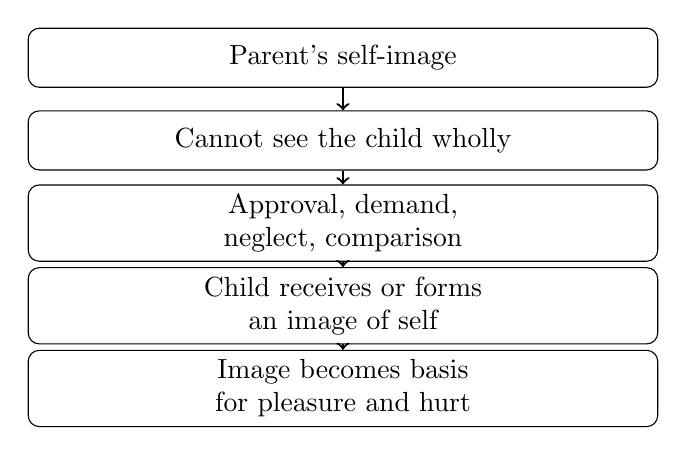
\begin{tikzpicture}[
  node distance=1.05cm,
  box/.style={draw, rounded corners, align=center, text width=0.64\linewidth, minimum height=0.75cm},
  arrow/.style={->, thick}
]
\node[box] (parent) {Parent's self-image};
\node[box, below of=parent] (notsee) {Cannot see the child wholly};
\node[box, below of=notsee] (transmit) {Approval, demand,\\neglect, comparison};
\node[box, below of=transmit] (child) {Child receives or forms\\an image of self};
\node[box, below of=child] (hurt) {Image becomes basis\\for pleasure and hurt};

\draw[arrow] (parent) -- (notsee);
\draw[arrow] (notsee) -- (transmit);
\draw[arrow] (transmit) -- (child);
\draw[arrow] (child) -- (hurt);
\end{tikzpicture}
\end{figure}

This figure is a transcript-backed conceptual reconstruction. It is not a redrawn blackboard diagram.

\section{Relationship Or No Relationship}

The lecture's relational claim is its hardest edge. If parent and child, husband and wife, friend and friend, or society and individual meet through images, is that relationship? Krishnamurti resists the softer phrase ``wrong relationship.'' He presses the division: relationship or no relationship.

Let us name the two cases:

\begin{align}
R_{\mathcal{I}} &= \text{relation governed by images}, \\
R_{\text{actual}} &= \text{relationship not governed by image}.
\end{align}

The first contrast is modest:

\begin{equation}
R_{\mathcal{I}} \neq R_{\text{actual}}.
\end{equation}

The lecture's stronger claim is more severe:

\begin{equation}
\mathcal{I}_{\text{self}} \neq \varnothing
\Rightarrow
R_{\text{actual}} = \varnothing.
\end{equation}

We should read this carefully. It is not a formal theorem. It is a compact notation for the claim under examination: as long as I have an image about myself, my relation with another is mediated by that image. I may play with words, sentiment, memory, and moments of warmth, but the image governs the field.

The rope analogy gives this its force. A person tied to a rope may move freely within a certain radius. He may say, ``At this moment I can move wherever I like.'' But the freedom is conditional. If he continues, he reaches the end of the rope, or the rope is yanked. In the same way, a person may have moments that feel like relationship, until the image is touched.

\begin{figure}
\centering
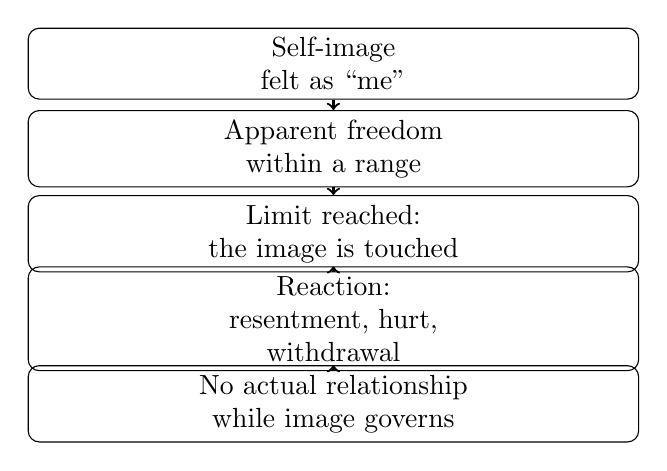
\begin{tikzpicture}[
  node distance=1.08cm,
  box/.style={draw, rounded corners, align=center, text width=0.62\linewidth, minimum height=0.75cm},
  arrow/.style={->, thick}
]
\node[box] (image) {Self-image\\felt as ``me''};
\node[box, below of=image] (range) {Apparent freedom\\within a range};
\node[box, below of=range] (limit) {Limit reached:\\the image is touched};
\node[box, below of=limit] (reaction) {Reaction:\\resentment, hurt,\\withdrawal};
\node[box, below of=reaction] (norel) {No actual relationship\\while image governs};

\draw[arrow] (image) -- (range);
\draw[arrow] (range) -- (limit);
\draw[arrow] (limit) -- (reaction);
\draw[arrow] (reaction) -- (norel);
\end{tikzpicture}
\end{figure}

This figure is also a conceptual reconstruction from the transcript. No screenshot evidence exists for a board diagram.

The discussion does not glide over the difficulty. A participant admits resentment at the statement. He remembers times that felt like relationship. Yet he also recognizes the ``yank back.'' That admission is part of the lecture's rhythm. The claim lands because resistance to it is heard, not ignored.

\subsection{Question \& Answer}

\paragraph{Question.}
If there are moments of affection or openness, why say there is no relationship?

\paragraph{Answer.}
The rope analogy answers this locally. A moment inside the range of the rope is not freedom from the rope. Likewise, a moment in which the image is not challenged is not freedom from image. If the image takes over when its limit is reached, then the image was the governing factor in reserve. The lecture's distinction is therefore not between good relationship and bad relationship, but between relationship and image-governed relation.

\section{Can The Machinery Stop?}

The final movement collects the whole inquiry into the question of consciousness. The speakers say that the content of consciousness makes up consciousness, and one of its major contents is image-making. We can write this as working notation, not as a metaphysical axiom:

\begin{equation}
\mathcal{C} \equiv \text{content of consciousness},
\qquad
\mathcal{I} \subset \mathcal{C}.
\end{equation}

Now the machinery is named. The image is the product of thought.

\begin{equation}
\text{image-making} = \text{product of thought}.
\end{equation}

Thought produces images of religion, nation, caste, tradition, superiority, inferiority, virtue, success, failure, and spiritual attainment. These images divide. Division destroys relationship. Where relationship is not actual, love becomes verbal, sentimental, romantic, or fanciful, but not the actuality under inquiry.

\begin{equation}
\text{thought} \to \text{image} \to \text{division} \to \text{no love}.
\end{equation}

Therefore the question is no longer merely, ``Why are we hurt?'' It is: can the machinery of image-making stop? Not occasionally. Not as a flash. Can it stop?

The dialogue then raises a subtle obstacle. If one says, ``All we know is image-making,'' that very ``all'' may block the question. It makes stopping impossible in advance. But if the question is allowed to stand, then the next temptation is to ask how. Krishnamurti refuses the how.

\subsection{Question \& Answer}

\paragraph{Question.}
How can image-making stop?

\paragraph{Answer.}
The question ``how'' turns too quickly into method. Method becomes system, practice, repetition, and achievement. Then the mind has acquired a new image: the image of the one who is practicing, progressing, or becoming free of images. The lecture therefore refuses evidence, experience, explanation, and method when they function as images.

The movement offered is much simpler and more demanding: see the fact and remain with the fact.

\begin{align}
\mathcal{F} + \text{thought/commentary}
&\to \mathcal{I}_{\text{new}}, \\
\mathcal{F} + \text{no commentary}
&\to \text{transformation}.
\end{align}

The word ``transformation'' is not a mechanism. It should not be made into an operator or a promised result. It marks the lecture's statement that when the mind remains with the fact without thought interfering, there is transformation.

\begin{figure}
\centering
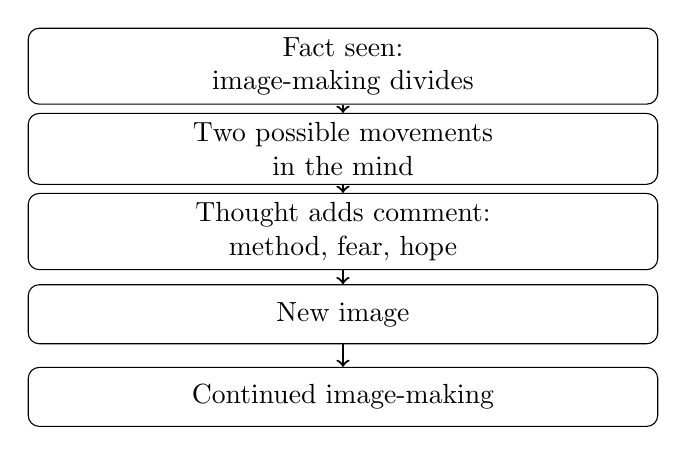
\begin{tikzpicture}[
  node distance=1.05cm,
  box/.style={draw, rounded corners, align=center, text width=0.64\linewidth, minimum height=0.75cm},
  arrow/.style={->, thick}
]
\node[box] (fact) {Fact seen:\\image-making divides};
\node[box, below of=fact] (fork) {Two possible movements\\in the mind};
\node[box, below of=fork] (comment) {Thought adds comment:\\method, fear, hope};
\node[box, below of=comment] (newimage) {New image};
\node[box, below of=newimage] (return) {Continued image-making};

\draw[arrow] (fact) -- (fork);
\draw[arrow] (fork) -- (comment);
\draw[arrow] (comment) -- (newimage);
\draw[arrow] (newimage) -- (return);
\end{tikzpicture}
\end{figure}

\begin{figure}
\centering
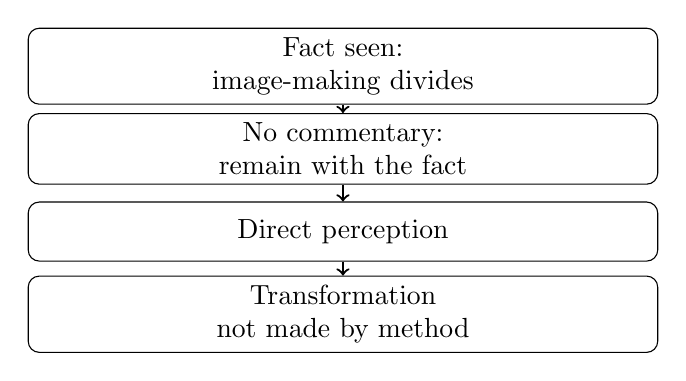
\begin{tikzpicture}[
  node distance=1.05cm,
  box/.style={draw, rounded corners, align=center, text width=0.64\linewidth, minimum height=0.75cm},
  arrow/.style={->, thick}
]
\node[box] (fact) {Fact seen:\\image-making divides};
\node[box, below of=fact] (stay) {No commentary:\\remain with the fact};
\node[box, below of=stay] (see) {Direct perception};
\node[box, below of=see] (trans) {Transformation\\not made by method};

\draw[arrow] (fact) -- (stay);
\draw[arrow] (stay) -- (see);
\draw[arrow] (see) -- (trans);
\end{tikzpicture}
\end{figure}

These two diagrams are split vertically for pocket layout. Together they reconstruct the transcript's final distinction: fact plus thought becomes another image; fact without commentary is the opening in which transformation is said to occur.

The lecture closes with restraint. If consciousness is filled with images, conclusions, ideas, and running away, what is consciousness when there is no image-making? The question is not answered here. It is left for the next inquiry.

\section{Summary}

The lecture begins with the problem of human change and immediately questions the inherited category of the unconscious. The word may already divide what is actually one movement of consciousness. What is called hidden may be a fact avoided, repeated avoidance made habitual, and a wound that remains.

The inquiry then turns to hurt. Hurt brings resistance, withdrawal, isolation, and the picture of oneself as hurt. The central discovery is that the image of oneself is what gets hurt. Because the image is felt as ``me,'' pleasure and pain are both attributed to me. The same image that gives pleasure can be wounded; it cannot be made to yield pleasure only.

The discussion then asks where image-making begins. It moves through child, parent, security, neglect, and society without importing an outside theory. The transcript's claim is narrower and more exact: where the parent or society acts through image, the child receives image; the image then becomes the basis of hurt.

The relational consequence is severe. Image-governed relation is not actual relationship. The rope analogy clarifies why moments of apparent freedom do not prove freedom from the image. When the limit is reached, the image takes over.

The final question is whether the machinery can stop. Image-making is identified as the product of thought, and thought-made images divide human beings and destroy relationship. The lecture refuses the expected ``how,'' because method would become another image. It ends with the demand to remain with the fact without commentary, and with the open question: what is consciousness when image-making is absent?